% Szglab4
% ===========================================================================
%
\chapter{Analízis modell kidolgozása 1}

\thispagestyle{fancy}

\section{Objektum katalógus}

\subsection{Glue}
A „Glue” objektum megvalósít egy adott tulajdonságú akadályt. Amely robot belemegy, annak a sebességét megfelezi. Ez az akadály eltünik, ha négyszer rálépnek.
\subsection{GUI}
A grafikus felületet megvalósító objektum. Ez az objektum maga a menü ami a játék indítása után ugrik fel, itt találhatóak a beállítások (mint például a gondolkodás idő és a maximális játék idő vagy a körök száma) és a játékmódok. Gombnyomásra fogja elindítani a játék működési szálát. Ez az objektum kezeli az ablak eseményeit és a játék bezárását.
\subsection{HUD}
Ez az objektum követi és nyilvántartja, hogy a robotok hány checkpoint-on mentek át, mennyi olaj és ragacs van náluk amit felhasználhatnak, illetve kiírja a képernyőre a hátramaradó időt és a megtett körök számát. Feladata, hogy minden körben megvizsgálja, hogy a robotok elérték-e a következő checkpointot.
\subsection{MapBuilder}
Fájlból beolvassa és létrehozza a memóriában a pályát, a kezdő pozíciókat és a checkpointokat reprezentáló objektumokat.  Mivel a  MapBuilder objektum tárolja a pályát így feladat, hogy vizsgálja a robotok azon belül tartózkodását.  
\subsection{Obstacle}
Az Obstacle absztrakt osztály, mely a Unit osztályból származik le. Ez az osztály fogja összefogni a pályán található (lerakott) akadályokat és bevezet egy absztrakt függvényt, ami a leszármazottakban implementálva érvényesíti hatását (lassítás, csúszás) egy robotra.
\subsection{Oil}
Ez az objektum az Obstacle osztály leszármazottja. Hasonlóan a Glue objektumhoz, egy adott hatást valósít meg, ami letiltja a következő körben történő irányítását a robotnak, ami belelépett. Az olaj felszárad meghatározott kör eltelte után.
\subsection{Phoebe}
A játék logikát megvalósító objektum. Listában tárolja a pályán tartózkodó robotokat, akadályokat és figyeli, hogy mikor ér véget a játék. A „Phoebe” objektumrajzolja ki az objektumokat a pályán és szálként indítható osztályt, melyben maga a játék fut. Játékindításkor berakja a pályára a robotokat és az akadályokat a kezdő pozíciókba. Ebben az objektumbantörténnek az ellenőrzések (akadályba vagy robotba ütközések, pályáról leesés).
\subsection{Robot}
Olyan objektum, mely a pályán található robotokat valósítja meg. Leírja a viselkedésüket és a kezelésüket. A „Robot” osztály a Unit-ból származik le, ezáltal van pozíciója és az ütközés is le van kezelve. Felelős a mozgásért, megállapítja egy adott akadállyal vagy robottal ütközött-e és kezeli a felhasználó által leütött gombokat.

\subsection{MyTimer}
Az eltelt időt és a fennmaradt idő nyilvántartásáért felelős. Ilyen például a játék elején három másodperces visszaszámlálás vagy a időlimites játékmód esetén, amikor a maximális időtől számol visszafelé. 
\subsection{Unit}
A Unit absztarkt osztály a pályán található objektumoknak a szülőosztálya. Tárolja a pozíciót, egy sokszöget, amivel vizsgálható az ütközés és a pályán megjelenő képüket. Továbbá ez az osztály valósítja meg a függvényt, ami ellenőrzi azt, ha két Unit ütközik (robotok egymással, robot akadállyal).

\subsection{Cleaner}
TODO
\subsection{MyListener}
A játék keylistener-jét megvalosító osztály. Külön szálon fut, hogy az egyszerre lenyomott gombok ne okozhasanak problémát. A játékban részvevő robotok KeyPressed függvényét hivogatja, a megfelelő KeyEvent paraméterrel.
\section{Osztályok leírása}


\subsection{GUI}
\begin{itemize}
\item Felelősség\\
A grafikus felületért felelős osztály, mely a menüt és a játékot megjeleníti.
\item Attribútumok
	\begin{itemize}
		\item \textbf{Phoebe} game: referencia a játékra
	\end{itemize}
\item Metódusok
	\begin{itemize}
		\item\textbf{GUI}(): Konstruktor. Beállítja az ablak nevét, létrehozza az ablak elemeit, elrendezi őket és beállítja a figyelőket(ActionListener).
	\end{itemize}
\end{itemize}

\subsection{HUD}
\begin{itemize}
\item Felelősség\\
A robotok ragacs- és olajkészletét, illetve megtett köreit és checkpontjait számolja. Megvalósítja a checkpoint ellenőrzést.
\item Attribútumok
	\begin{itemize}
		\item \textbf{int[]} checkpointReached: Minden robothoz külön tárolja a legutoljára érintett checkpoint sorszámát.
		\item \textbf{int[]} lap: Minden robothoz tárolja a megtett körök számát. 
		\item \textbf{int[]} numGlue: Minden robothoz tárolja a ragacsok számát.
		\item \textbf{int[]} numOil: Minden robothoz tárolja az olajok számát.
		\item \textbf{List<Shape>} checkpoints: Tárolja a checkpointokat reprezentáló objektumokat List adatszerkezetben. A checkpointSearch függvény kérdezi le ebből a következő checkpoint helyzetét. 
		\item \textbf{List<Robot>} robots: A robotokat tároló List adatszerkezet. A checkpointSearch függvény kérdezi le ebből a robotokat, majd azok helyzetét.
	\end{itemize}
\item Metódusok
	\begin{itemize}
		\item \textbf{HUD}(List<Robot> robs): Konstruktor, inicializálja a köröket számláló változót, az érintett checkpointokat, a ragacs és olajkészleteket. 
		\item void \textbf{checkpointSearch}(): Ellenőrzi hogy a robotok teljesítették-e a következő checkpointot.
		\item void \textbf{setCheckpoints}(List<Shape> checkObj): Checkpointokat reprezentáló adatszerkezet betöltése.
		
	\end{itemize}
\end{itemize}

\subsection{MapBuilder}
\begin{itemize}
\item Felelősség\\
A pálya felépítéséért, a checkpointok tárolásáért és a robot pályán tartózkodásának vizsgálatáért felelős osztály.
\item Attribútumok
	\begin{itemize}
		\item \textbf{Shape} map: A pályát reprezentáló objektum. 
		\item \textbf{List<Shape>} checkpoints: Tárolja a checkpointokat reprezentáló objektumokat List adatszerkezetben.
		\item \textbf{int[]} startPosPlayerOne: Meghatároz egy (x,y) koordinátát, ahol az első játékos kezd.
		\item \textbf{int[]} startPosPlayerTwo: Meghatároz egy (x,y) koordinátát, ahol az második játékos kezd.
	\end{itemize}
\item Metódusok
	\begin{itemize}
		\item \textbf{MapBuilder}(): Konstruktor, a pálya beolvasása fájlból, majd létrehozása.
		\item boolean \textbf{fallingDown}(Shape othershape): Igaz értéket ad vissza, ha a robot leesett a pályáról, hamisat ha még rajta van.
	\end{itemize}
\end{itemize}


\subsection{MyListener}
\begin{itemize}
\item Felelősség\\
A külön szálon futó KeyListener-t megvalósító osztály.
\item Interface-ek:\\
    \begin{itemize}
    \item KeyListener
    \item Runnable
    \end{itemize}
\item Attribútumok
	\begin{itemize}
		\item \textbf{boolean} isUp: Azt tárolja, hogy le van-e nyomva a felfele nyil.
    	\item \textbf{boolean} isDown: Azt tárolja, hogy le van-e nyomva a lefele nyil.
    	\item \textbf{boolean} isRight:Azt tárolja, hogy le van-e nyomva a jobbra nyil.
    	\item \textbf{boolean} isLeft:Azt tárolja, hogy le van-e nyomva a balra nyil.
    	\item \textbf{boolean} isW:Azt tárolja, hogy le van-e nyomva a W a billentyűzeten.
    	\item \textbf{boolean} isD:Azt tárolja, hogy le van-e nyomva a D a billentyűzeten.
    	\item \textbf{boolean} isS:Azt tárolja, hogy le van-e nyomva az S a billentyűzeten.
    	\item \textbf{boolean} isA:Azt tárolja, hogy le van-e nyomva az A a billentyűzeten.
   	\item \textbf{List<Robot>} robots: Azon robotok listája akiknek a keyPressed függvényét kell hívnia.
	
	
	\end{itemize}
\item Metódusok
	\begin{itemize}
		\item \textbf{MyListener}(List<Robot> r): beállítja a lenyomott gombokat figyelő változókat false-ra , továbbá beállítja a robots változó referenciáját a paraméterként kapotra.
			\item void\textbf{keyPressed}(KeyEvent e): Beállítja a lenyomot gombokat figyelő változók küzül a Keyeventnek megfelelőt  true-ra , ha meg nyomták valamelyiket  a figyelt gombok közül.
			\item void\textbf{keyReleased}(KeyEvent e): Beállítja a lenyomot gombokat figyelő változók küzül a Keyeventnek megfelelőt false-ra , ha fel engedték valamelyiket a figyelt, lenyomott gombok közül.
				\item void\textbf{run}(): Végtelen ciklust futtat. Megvizsgálja hogy melyik gombok vannak lenyomva, majd a nekik megfelelő KeyEvent-tel paraméterezve meghívja a hozzátartozó robotoknak a Keypressed függvényét. Majd alszik a szál 30 mili secundomig.
	\end{itemize}
\end{itemize}


\subsection{Obstacle}
\begin{itemize}
\item Felelősség\\
A pályán/játékosoknál lévő különböző akadályokat (ragacs,olaj) összefogó ősosztály.
\item Ősosztályok\\
Unit
\item Attribútumok
	\begin{itemize}
		\item \textbf{int} WIDTH: Az akadályokat jellemző szélesség. Szükség van rá, hogy létrehozzuk a leszármazottak hitbox-át(sokszög pályaelem).
		\item \textbf{int} HEIGHT: Az akadályokat jellemző hosszúság. Szükség van rá, hogy létrehozzuk a leszármazottak hitbox-át(sokszög pályaelem).
			\item \textbf{int} lifetime: Generikussan az akadályok életben maradásának ellenörzésére szolgál. Olaj esetében megadja, hogy hány kör telt el az akadály lerakása óta. Ragacs esetében pedig, hogy hányan léptek rá mióta lekerült. 
	\end{itemize}
\item Metódusok
	\begin{itemize}
		\item \textbf{Obstacle}(int x, int y): meghívja a Unit konstruktorát a megadott adatokkal és létrehoz egy négyzet elemet ami reprezentálja a pályán majd.
		\item void \textbf{effect}(Robot r): Meghatározza, milyen hatással van a robotra, ha érintkezik egy Obstacle-lel. Absztrakt.
		\item boolean \textbf{checkAlive}():Az akadályok vizsgálata amit a játékmotor minden körben meghív minden akadályra. Absztrakt.
	\end{itemize}
\end{itemize}

\subsection{Glue}
\begin{itemize}
\item Felelősség\\
A játékban szereplő Ragacs foltok viselkedését leíró osztály
\item Ősosztályok\\
Unit$\rightarrow$Obstacle
\item Attribútumok
	\begin{itemize}
		\item \textbf{BufferedImage} img: Ez a privát statikus atribútum a ragacs képét tárolja,                                      a megjelenítésben van szerepe.
	\end{itemize}
\item Metódusok
	\begin{itemize}
		\item  \textbf{Glue}(int x,int y):A ragacs konstruktora, meghívja az őse (obstacles)                           konstruktorát x,y paraméterrel, továbbá beállítja a lifetime-ot 4-re.
		
		\item void \textbf{effect}(Robot r): Ütközéskor hívja meg az ütközést vizsgáló függvénye     a Robot osztálynak. Módosítja a robot slowed értékét a 50\%-ra a robot slowed attribútum         setterének meghívásával. Továbbá csökkenti a ragacs élettartalmát egyel.
	
		\item boolean \textbf{checkAlive}():A játékmotor hívja meg minden kör végén, ha a lifetime értéke>0 true-val tér vissza, különben false-al.
			\item void \textbf{paint}(Graphics2D g):Kirajzolja a ragacs képét az x,y koordinátákon.
				\item void \textbf{setUnitImage}():Beállítja a ragacs osztályhoz tartozó képet a user directoryban található glue.jpg-re
			\item String \textbf{toString}()Vissza ad egy stringet a  ragacs legfontosabb értékeivel.(x, y, WIDTH, HEIGHT, lifetime)
		
	\end{itemize}
\end{itemize}

\subsection{Oil}
\begin{itemize}
\item Felelősség\\
A pályára lerakható olaj megvalósítása. Ha belelép egy játékos egy ilyen olajfoltba az effect függvény letiltja a mozgatást az adott roboton a következő ugrásig.
\item Ősosztályok\\
Unit $\rightarrow$ Obstacle 
\item Attribútumok
	\begin{itemize}
		\item \textbf{BufferedImage} img: Ez a privát statikus atribútum az olaj képét tárolja,  a megjelenítésben van szerepe.
	\end{itemize}
\item Metódusok
	\begin{itemize}
		\item \textbf{Oil}(int x, int y): Egy Oil elem létrehozásáért felelős. Meghívja az ős konstruktorát x,y-paraméterrel, továbbá beállítja a lifetime-ot default értékre.
		\item void \textbf{effect}(Robot r): Meghatározza, milyen hatással van a robotra, ha beleugrik egy olajfoltba. Ebben az esetben letiltja a játékost, hogy irányt váltson.
			\item void \textbf{setUnitImage}():Beállítja az olaj osztályhoz tartozó képet a user directoryban található oil.jpg-re
				\item boolean \textbf{checkAlive}():A játékmotor hívja meg minden kör végén, lifetime értékét csökkenti 1 el, ha a lifetime értéke>0 (csökkentés után)true-val tér vissza, különben false-al.
		\item String \textbf{toString}()Vissza ad egy stringet az olaj legfontosabb értékeivel.(x, y, WIDTH, HEIGHT, lifetime)
	\end{itemize}
\end{itemize}

\subsection{Phoebe}
\begin{itemize}
\item Felelősség\\
A játék motorját megvalósító objektum. Listában tárolja a pályán tartózkodó robotokat,kisrobotokat, akadályokat és 
 figyeli, hogy mikor ér véget a játék. A „Phoebe” objektum rajzolja ki az objektumokat a pályán és 
 szálként indítható osztályt, melyben maga a játék fut. Játékindításkor berakja a pályára a robotokat és 
 az akadályokat a kezdő pozíciókba. Ebben az objektumban történnek az ellenőrzések (akadályba vagy 
  robotba ütközések, pályáról leesés)
  \item Interface:
  \begin{itemize}
  \item Runnable
  \end{itemize}
\item Attribútumok
	\begin{itemize}
		\item \textbf{boolean} ended: Állapot változó, ha vége a játéknak, akkor true. Ha beteljesül egy játék végét jelentő esemény, akkor ezen a változón keresztül leáll a játék és megállapítódik a nyertes.
		\item \textbf{BufferedImage} background: A játék hátterét adó kép.
		\item \textbf{List<Robot>} robots: A játékban szereplő robotok listája.
		\item \textbf{List<Obstacle>} obstacles: A játékban szereplő akadályok listája.
		\item \textbf{HUD} hud: A játékosok előrehaladását, ragacs és olajkészleteit tartja számon
		\item \textbf{MapBuilder} map: TODO
		\item \textbf{Settings} gameInfo:A játék beállításait tartalmazza         \item \textbf{List<Cleaner>} cleaners: A játékban lévő aktív kis tisztogató robotokat tartja számon.
        \item \textbf{MyTimer} gameTimer: A játékban futó óra, ami visszaszámlálásoknál és a játék végének meghatározásánál játszik szerepet.

		
			
	\end{itemize}
\item Metódusok
	\begin{itemize}
		\item \textbf{Phoebe}(Setting set): A játék felépítése, a robotok,a tisztogató kisrobotok és  az akadályok listáinak létrehozása.Az ended inicializálása ,az init függvény meghívása és a grafikus felület felépítése történik itt.
		\item void \textbf{run}(): Ez a metódus futtatja a főciklust, amelyben maga a játék működik.
	\item void \textbf{Paint}(Graphics2D g2d): Kirajzolja a játék aktuális állását. 
	\item void \textbf{addObstacle}(Obstacle item): Hozzá ad egy Obstacle-t a játékban lévők listájához.
	
	\item void \textbf{init}(): Inicializálja a játékot a kezdeti beállításokra. Létrehozza az időzítőt, a mapot, a robotokat a kezdőpozíciók szerint,a hudot és beállítja a különböző osztályokhoz tartozó statikus képeket, továbbá a pálya alap ragacsait és olajait is szétszórja.
	\end{itemize}
\end{itemize}

\subsection{Robot}
\begin{itemize}
\item Felelősség\\
A játékban résztvevő robotok viselkedését és kezelését leíró osztály.
\item Ősosztályok\\
Unit

\item Attribútumok
	\begin{itemize}
		\item \textbf{int} staticID: Az osztályhoz tartozó statikus azonosító, a példány                azonosítójának(id) meghatározásához szükséges.
			\item \textbf{static final int} r: Az ugrás számításához tartozó sugár. 
				\item \textbf{static int} ANIMATIONSPEED: Az ugrás animálásának részletessége(hányszor hívja meg a paintet). 
		\item \textbf{static int} HEIGHT: A robot képének magassága, collision                      detektálásnál, továbbá az irányítást segítő nyíl kezdő koordinátájának                  meghatározásánál szükséges.
		\item \textbf{static int} WIDTH:A robot képének szélessége, funkcionalitásban hasonló a WIDTH-hez.
		\item \textbf{int} ID: A robot példányának egyedi azonosítója, a keyconfig sorának                     indexelésére és a collison detektálásnál az önmagával való ütközés                      kivédésére szükséges.
		\item \textbf{int} numGlue:A robotnál lévő ragacskészletet tárolja.
		\item \textbf{int} numOil:A robotnál lévő olajkészletet tárolja.
		\item \textbf{boolean} leftobstacle:Megmondja hogy raktunk-e már le ebben a körbe olajat vagy ragacsot kezdő érték false, minden lépés után vissza áll false ra és minden obstacle lerakásnál true ra .
	\item \textbf{BufferedImage}img[]:A robotok képeit tartalmazza,az animáció miatt többet.
	
		\item \textbf{double} slowed: A sebesség modosításáért felel, default értéje 1.0, amennyiben ragacsba lép a robot ez 0.5-re módosul és minden ugrás végén visszaáll az eredeti értékére, ugrásnál ezzel szorozzuk be a végkordinátát kiszámító sugár hosszát.
		\item \textbf{boolean} oiled: Azt jelzi, hogy olajba lépett-e, ennek hatására a mozgás iránya módosíthatatlanná válik egy kis időre. 
		\item \textbf{int} arrowendx: A robot irányítását segítő nyilnak az x koordinátája, a nyíl kirajzolásánál van szerepe.
		\item \textbf{int} arrowendy: A robot irányítását segítő nyilnak az y koordinátája, a nyíl kirajzolásánál van szerepe.
		\item \textbf{double} alpha: A robot irányítását segítő nyíl vízszintessel bezárt szöge. A nyil kirajzolásánál, az ugrás végpontjának meghatározánál van szerepe.
		\item \textbf{boolean} moved: Azt jelöli, hogy lépett-e már a robot az aktuális körben. A megjelenítésnél(nyilat ugrás közben nem jelenítjük meg),illetve az irányítás letiltásánál van szerepe(olajba lépés esetén).
	
\end{itemize}
\item Metódusok\\
	\begin{itemize}
		\item \textbf{Robot}(int x,int y,Phoebe p): Létrehoz egy robotot a megadott x,y kordinátákon, inicializálja a tagváltozóit és eltárolja a játékmotor referenciáját.
		\item void\textbf{deathanimation}():A Robot halálának gafikus megjelenítéséért felelős függvény.
		\item void\textbf{setOiled}():Az oiled értékét true-ra állítja. 
		\item void\textbf{setGlued}():A slowed értékét 0.5-re állítja. 
		\item int\textbf{getId}():A Robot id-ét adja vissza.
		\item int\textbf{getNumGlue}():Visszatér a felhasználható ragcsok számával.
		\item int\textbf{getNumOil}():Visszatér a felhasználható olajok számával.
		\item void\textbf{incNumOil}():Növeli a robotnál tárolt olajok számát, ha az nem haladja meg a 3 at.
		\item void\textbf{incNumGlue}():Növeli a robotnál tárolt ragacsok számát, ha az nem haladja meg a 3 at.
	\item void\textbf{paint}(Graphics2D g):kirajzolja a robotot a saját koordinátáin, ha nem lép éppen akkor az irányítást segítő nyilat is.
	\item void\textbf{setUnitImage}():beállítja a robot osztályhoz tartozó képeket.
\item void\textbf{bounce}():A robotok ütközésekor a lepattanás céjának  koordinátáinak számolása történik itt.

		\item void\textbf{move}():A robot mozgatásáért és annak leanimálásáért felelős függvény.Kiszámolja az új koordinátát és oda ugrasztja a robotot, majd frissíti a hitboxot.
		\item boolean \textbf{collisionWithObstacle}(Obstacle o): Ellenőrzi hogy a robot ütközött-e az akadállyal, igazzal tér vissza ha igen, hamissal ha nem.
		\item void \textbf{collisionWithRobot}(Robot r): Ellenőrzi hogy a robot ütközött-e másik robottal ,  referencia alapján kiszüri ha önmagára hívják meg.Ha volt ütközés meghívja a bounce függvényt önmagára.
		\item void \textbf{keyPressed}(int e):A robot irányítását megvalósító függvény, a játékmotor keylistener-e által hívódik meg, a lenyomott billentyű azonosítójával. A következő ugrás beállítása, a ragacs/olaj lerakása történhet itt. A Settings.keyconfig változó felhasználásával.
				\item String \textbf{toString}()Vissza ad egy stringet a robot legfontosabb értékeivel.(id, slowed, oiled, x, y, nextx, nexty, alpha, WIDTH, HEIGHT, numGlue, numOil)
	\end{itemize}
\end{itemize}

\subsection{Timer}
\begin{itemize}
\item Felelősség\\
A visszaszámlálásért (idő, director time) felelős.
\item Metódusok
	\begin{itemize}
		\item \textbf{Timer}(int i): Konstruktor, inicializál egy viszaszámláló órát.
		\item boolean \textbf{isZero}(): Igazzal tér vissza ha a megadott idő lejárt;
	\end{itemize}
\end{itemize}

\subsection{Unit}
\begin{itemize}
\item Felelősség\\
A pályán található objektumokért felel és azok viszonyáról (például ütközésükről).
\item Attribútumok
	\begin{itemize}
		\item \textbf{int} x: Az egység x koordinátája
		\item \textbf{int} y: Az egység y koordinátája
		\item \textbf{Rectangle} hitbox: Az egységet a pályán reprezentáló sokszög.
	\end{itemize}
\item Metódusok
	\begin{itemize}
		\item void \textbf{move}() : Absztrakt függvény, mely a leszármazottakban fog megvalósulni. Az egységek mozgásáért felelős.
		\item boolean \textbf{intersect}(Unit u): Két egység ütközését meghatározó függvény.
	\end{itemize}
\end{itemize}
\pagebreak
\section{Statikus struktúra diagramok}

\begin{figure}[h]
\begin{center}
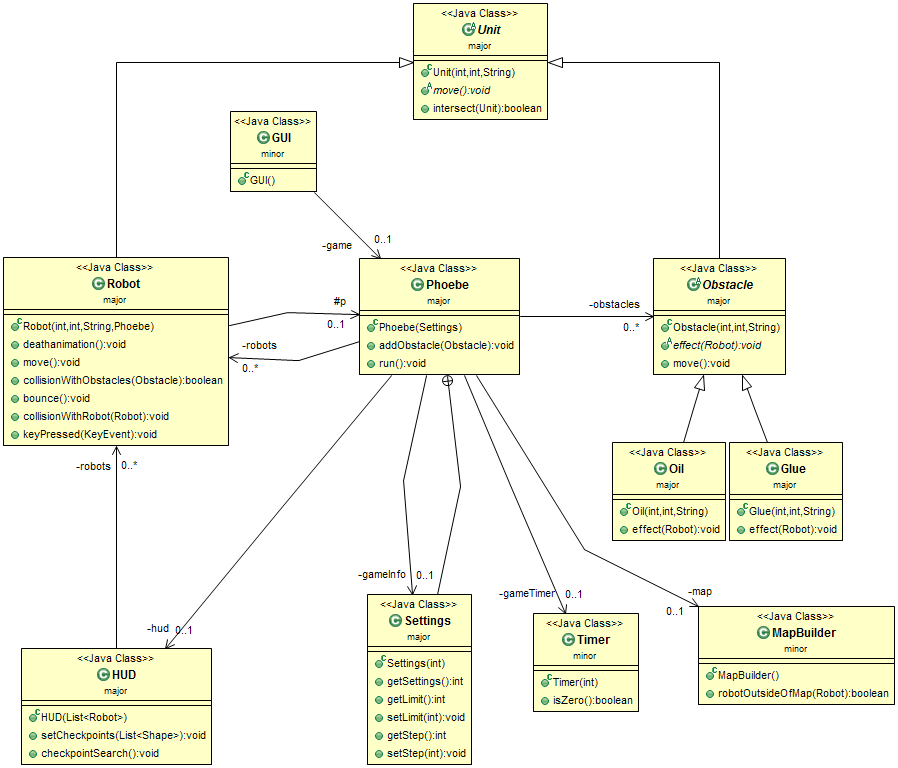
\includegraphics[width=17cm]{images/struktdiagram.PNG}
\caption{Statikus struktúra diagram}
\label{fig:example3}
\end{center}
\end{figure}
\pagebreak
\pagebreak

\section{Szekvencia diagramok}

\subsection{Robot::CheckpointSearch}
\begin{figure}[h]
\begin{center}
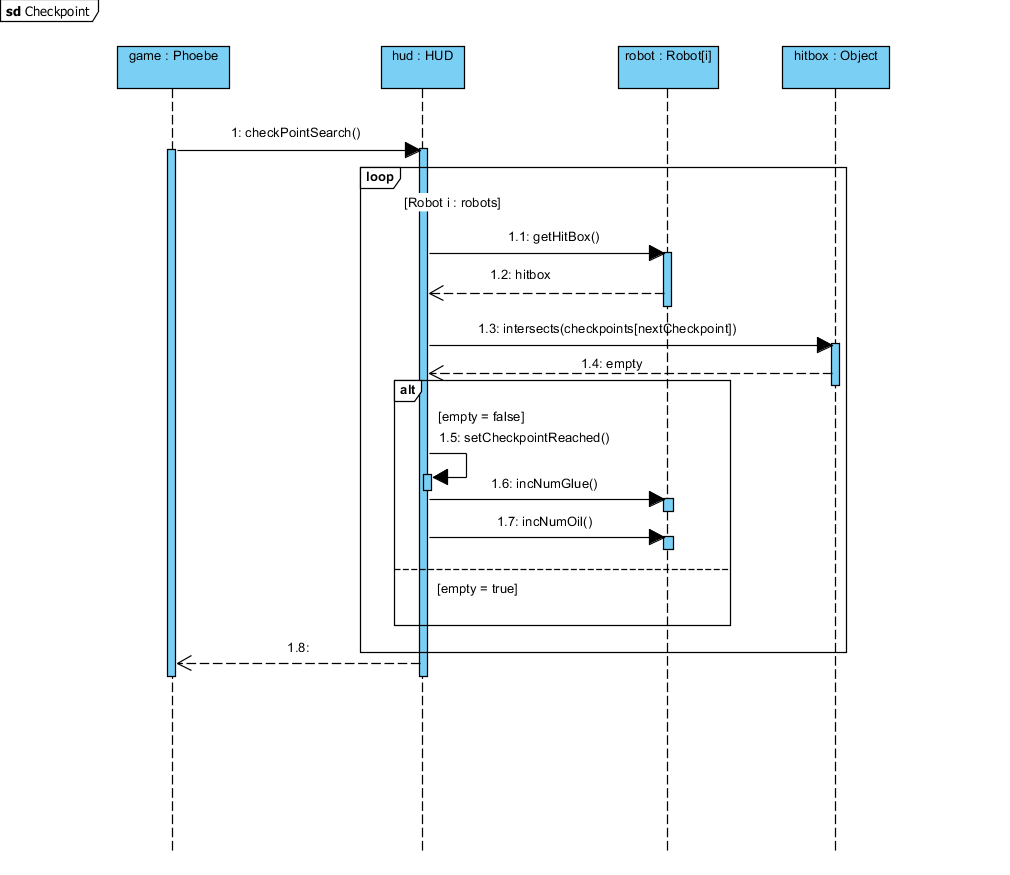
\includegraphics[width=17cm]{images/CheckpointSearch.PNG}
\caption{Következő checkpoint vizsgálata}
\label{fig:example2}
\end{center}
\end{figure}
\pagebreak

\subsection{Robot::CollisonWithObstacle}
\begin{figure}[h]
\begin{center}
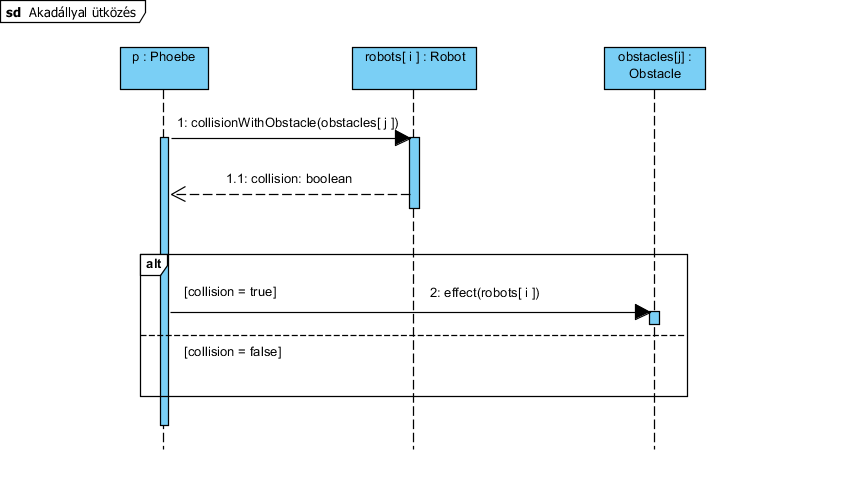
\includegraphics[width=17cm]{images/collisionWithObstacle()_sequence.PNG}
\caption{Robot ütközése akadállyal}
\label{fig:example4}
\end{center}
\end{figure}
\pagebreak

\subsection{Robot::CollisionWithRobot}
\begin{figure}[h]
\begin{center}
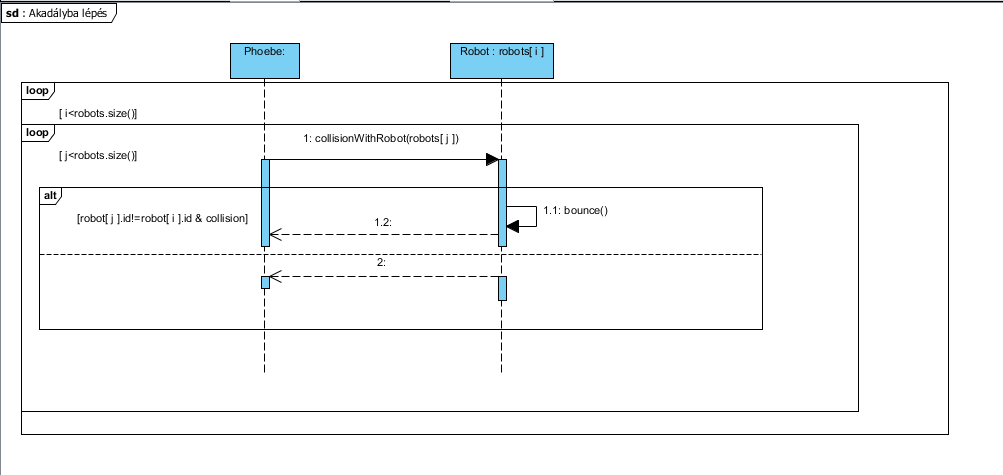
\includegraphics[width=17cm]{images/collisionWithRobot()_sequence.PNG}
\caption{Robot ütközése akadállyal}
\label{fig:example5}
\end{center}
\end{figure}
\pagebreak

\subsection{Robot::FallDown}
\begin{figure}[h]
\begin{center}
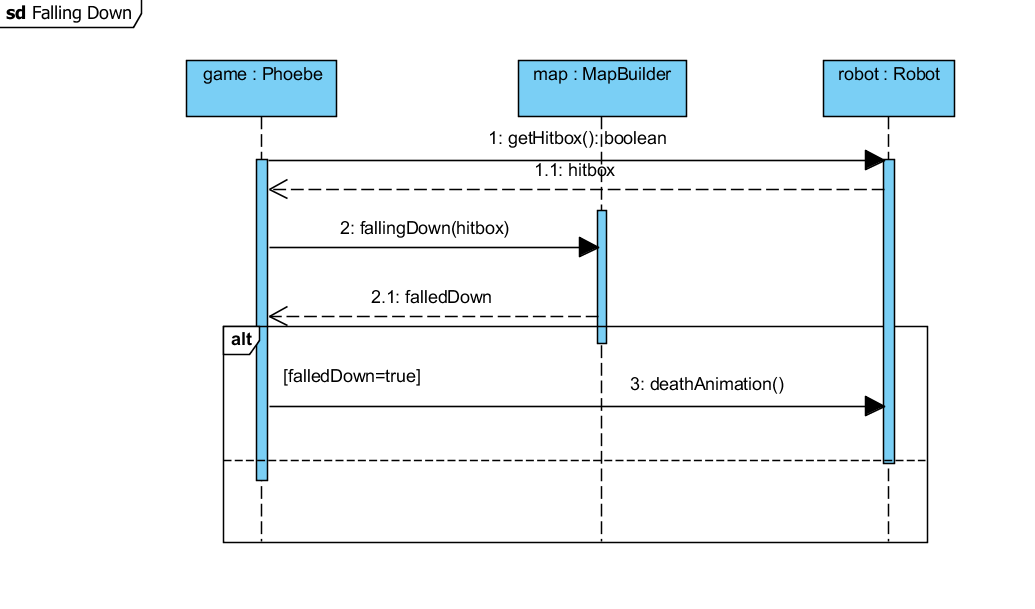
\includegraphics[width=17cm]{images/FallingDown.PNG}
\caption{Robot leesése a pályáról}
\label{fig:example6}
\end{center}
\end{figure}
\pagebreak

\subsection{Robot::InitGame}
\begin{figure}[h]
\begin{center}
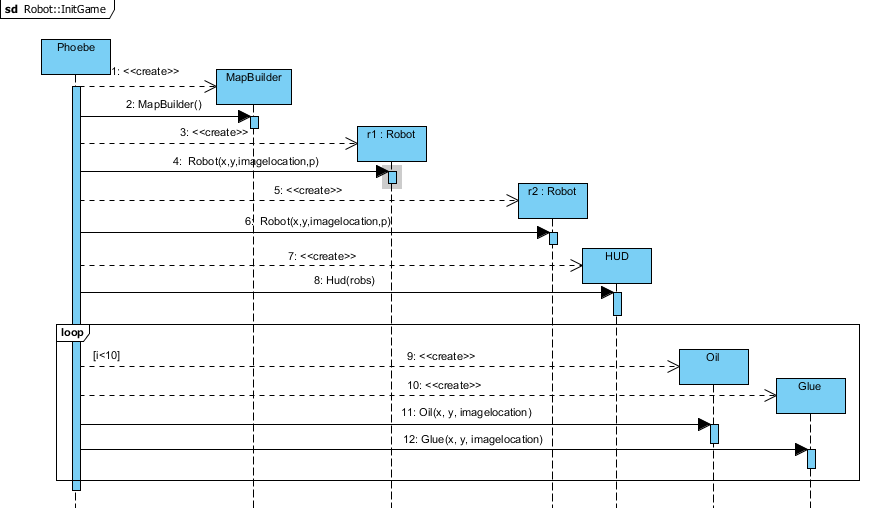
\includegraphics[width=17cm]{images/RobotInitGame.PNG}
\caption{A játék inicializálása}
\label{fig:example7}
\end{center}
\end{figure}
\pagebreak

\subsection{Robot::Move}
\begin{figure}[h]
\begin{center}
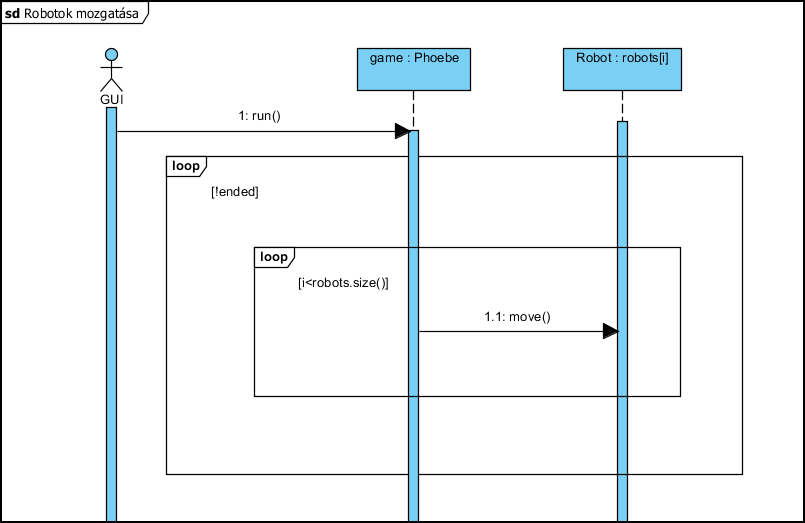
\includegraphics[width=17cm]{images/RobotMove.png}
\caption{A robot mozgatása}
\label{fig:example8}
\end{center}
\end{figure}
\pagebreak

\subsection{Robot::NewObstacle}
\begin{figure}[h]
\begin{center}
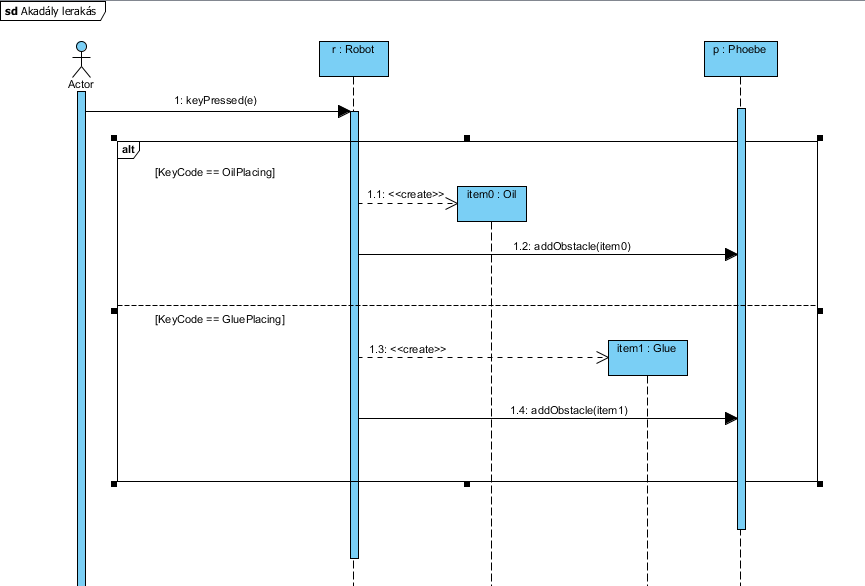
\includegraphics[width=17cm]{images/RobotAddObstacle.png}
\caption{Akadály lerakása}
\label{fig:example9}
\end{center}
\end{figure}
\pagebreak

\subsection{Robot::Settings}
\begin{figure}[h]
\begin{center}
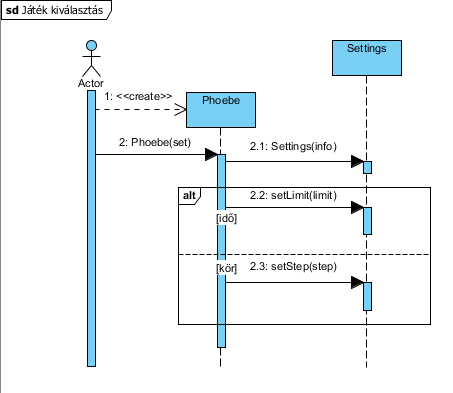
\includegraphics[width=17cm]{images/kivalasztas.PNG}
\caption{A játék beállításainak kiválasztása}
\label{fig:example10}
\end{center}
\end{figure}
\pagebreak

\subsection{Robot::End}
\begin{figure}[h]
\begin{center}
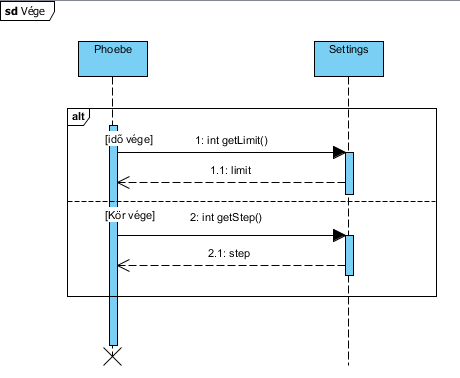
\includegraphics[width=17cm]{images/end.PNG}
\caption{Játék vége}
\label{fig:example11}
\end{center}
\end{figure}
\pagebreak



\section{State-chartok}
\subsection{Robot::States}
\begin{figure}[h]
\begin{center}
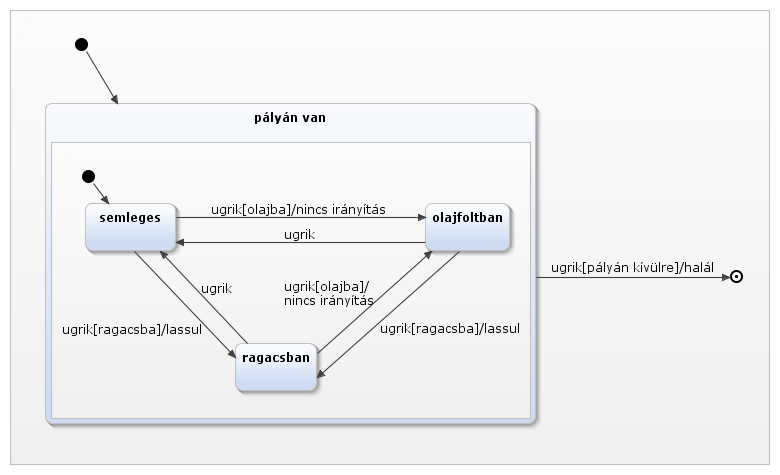
\includegraphics[width=17cm]{images/robot.png}
\caption{A robot állapotai}
\label{fig:example12}
\end{center}
\end{figure}

